\documentclass[a4paper,11pt]{jsarticle}


% 数式
\usepackage{amsmath,amsfonts}
\usepackage{amssymb,latexsym}
\usepackage{amsthm}
\usepackage{bm}
\usepackage{physics}
% 画像
\usepackage[dvipdfmx]{graphicx}
% ローマ数字
\usepackage{otf}
% 単位
\usepackage{siunitx}
% 表
\usepackage{multirow}
% 化学反応
\usepackage[version=4]{mhchem}

\theoremstyle{definition}
\newtheorem{thm}{定理}
\newtheorem{dfn}{定義}
\newtheorem{ex}{例}

\begin{document}

\title{2022年4月28日発表分の資料}
\author{齋藤駿一}
\date{\today 作成}
\maketitle

\begin{abstract}
  論文``The Chemical Thermodynamics for Growing Systems"についての1回目の発表をまとめました.
  2回目の発表(5月12日予定)の参考にしてください.
\end{abstract}

\tableofcontents

\section{論文の概要}
この論文の内容を一言で言えば,「生物のモデルになりそうな系の成長条件を,少ない仮定から熱力学的に導出した」となります.
具体的には,浴(reservoir)の中に膜で囲まれた系を用意し,膜を透過する物質と透過しない物質を仮定します.
系は浴と相互作用し,物質間では化学反応が起こります.
ただし,膜を透過しない物質の化学反応として,``autocatalytic core''と呼ばれる特別なものを考えています.
その結果,系のエネルギー,体積,各物質の粒子数が変化し,全系のエントロピーを最大化する方向に系の状態が遷移します.
論文では,この系をヘッセ幾何学を用いて解析することで,系が成長するための熱力学的条件を導出しています.

\section{発表の方針}
この論文についての発表は2回に分けて行います.
すでに行った1回目の発表では,まず``autocatalytic core''について説明した後,系を解析するための仮定をおき,系の状況を整理する途中まで終わりました.
2回目の発表では,その続きを行った後,ヘッセ幾何学を使うための準備を行い,最終的に系の成長条件を導く予定です.

\section{前提知識:``autocatalytic core"とは何か}
\subsection{単純な触媒反応との違い}
単純な触媒反応は,触媒Eが反応物Aと結合して中間体となり,Aを生成物Bに変えて解離するというものである:
\begin{equation}
  \ce{A + E <=> EA <=> B + E}
\end{equation}
このとき,反応の前後で触媒の総量は変わらない.
これに対し,自己触媒反応とは上の反応式で$\ce{E} = \ce{B}$とした
\begin{equation}
  \ce{A + B <=>[(a)] AB <=>[(b)] 2B} \label{autocatalysis}
\end{equation}
のように,触媒反応で触媒自身が生成される反応である.
自己触媒反応は生物の特徴的な反応である.
非常にざっくりとAを栄養,Bを細胞とみなせば,上の式は,反応(a)で細胞が栄養を取り込み,反応(b)で細胞が分裂するように見える\footnote{反応式\eqref{autocatalysis}のA,B,ABは分子なので,これはあまり良い例ではない.実際,生物が用いる自己触媒反応は反応式\eqref{autocatalysis}とは違う形のものがほとんどらしい.}.

\subsection{数学的な定義}
次に,autocatalytic coreを定義するために,自己触媒反応をもう少し数学的に取り扱う.

\begin{dfn}
  \label{reaction_graph}
  Reaction graphとは3つ組$(S,R,M)$のことである.ここで,
  \begin{itemize}
    \item $S$:化学種の集合(A,B,ABなど)
    \item $R$:反応の集合((a),(b)など)
    \item $M$:stoichiometric matrix\footnote{むりやり「化学量論的行列」と訳すのはやめた.} 
  \end{itemize}
  である.最後の$M$は行列であり,各行に$S$の元を,各列に$R$の元を対応させ,各成分$m_{ij}$を「反応$j$が順方向に1回進むことによる化学種$i$の粒子数変化」としたものである.
\end{dfn}
\begin{ex}
  先ほどの反応式\eqref{autocatalysis}の場合,1行目から順に化学種A,B,ABを対応させ,1列目から順に反応(a),(b)を対応させることで,
\begin{equation}
  M = \left( \begin{matrix}
    -1 & 0 \\
    -1 & 2 \\
    1 & -1 
  \end{matrix}
  \right)
\end{equation}
が得られる.
\end{ex}


また,反応の進行度はベクトルで表し,それを反応ベクトルと呼ぶ.
\begin{ex}
  反応式\eqref{autocatalysis}で反応(a)が2回,反応(b)が1回進んだ場合,反応ベクトルは
\begin{equation}
  \gamma = \left( \begin{matrix}
    2 \\
    1
  \end{matrix}\right)
\end{equation}
となり,このとき
\begin{equation}
  M \gamma = \left( \begin{matrix}
    -1 & 0 \\
    -1 & 2 \\
    1 & -1 
  \end{matrix}
  \right) 
  \left( \begin{matrix}
    2 \\
    1
  \end{matrix}\right)
  = \left(
    \begin{matrix}
      -2 \\
      0 \\
      1
    \end{matrix}
  \right)
\end{equation}
と計算できる.
これは,各行に対応する化学種の粒子数がどれだけ変化したかを表している.(Aは2個減って,Bが4個増えて,ABが1個増えている.)
このように,$M$を用いると反応の結果がシステマティックに分かる.
\end{ex}


次に,stoichiometric matrixに関する2つの用語を定義する.
\begin{dfn}
  $M$がproductiveであるとは,ある反応ベクトル$\gamma$があって,$M\gamma$のすべての成分が正となることである.(直観的に言い換えれば,「$M$に属するすべての化学種が一斉に増加するような反応の方向が存在する」ということである\footnote{この表現は発表時に古澤先生からいただいた言葉をもとにしている.}.)
\end{dfn}
\begin{ex}
  仮想的に
\begin{equation}
  M' = \left(
    \begin{matrix}
      1 & 0 \\
      -1 & 2 \\
      1 & -1
    \end{matrix}
  \right)
\end{equation}
をとると,反応ベクトル
\begin{equation}
  \gamma = \left(
    \begin{matrix}
      3 \\
      2
    \end{matrix}
  \right)
\end{equation}
に対して
\begin{equation}
  M'\gamma = \left(
    \begin{matrix}
      3 \\
      1 \\
      1
    \end{matrix}
  \right)
\end{equation}
となるので,$M'$はproductiveである.
一方で,$M$はproductiveではない.
\end{ex}

\begin{dfn}
  $M$がautonomousであるとは,$M$のすべての列に正の成分と負の成分が両方含まれていることである.
\end{dfn}
\begin{ex}
  見れば分かる通り,$M$も$M'$もautonomousである.
\end{ex}
以上より,autocatalytic coreが定義できる.
\begin{dfn}
  $M$がautocatalytic coreであるとは,次の二つが成り立つことである.
  \begin{itemize}
    \item $M$がproductiveかつautonomousである
    \item $M$の小行列\footnote{$M$の行または列のいくつかを取り除いて得られる行列のこと.}でproductiveかつautonomousであるものが存在しない
  \end{itemize}
\end{dfn}
つまり,autocatalytic coreとは,自己触媒反応の性質(productiveかつautonomous)をみたす最小のstoichiometric matrixであるといえる.
その意味で,autocatalytic coreは自己触媒反応の本質的な部分を取り出したものだと考えることができる.
\begin{ex}
  $M'$はproductiveかつautonomousだが,小行列としてとれる
\begin{equation}
  \bar{M} = \left(
    \begin{matrix}
      -1 & 2 \\
      1 & -1
    \end{matrix}
  \right)
\end{equation}
がproductiveかつautonomousなので,autocatalytic coreではない.
一方で,こうしてとった$\bar{M}$はautocatalytic coreである.
この$\bar{M}$は$M$の小行列でもあるので,自己触媒反応\eqref{autocatalysis}の代表的な部分といえる.
\end{ex}

加えて,autocatalytic coreの性質として次が知られている.
\begin{thm}
  Autocatalytic coreは正方行列であり,正則である.
\end{thm}
証明は省略するが,今回の論文ではこの正則性が非常に重要な役割を担う.

\section{系のセットアップ}
ここからいよいよ論文の説明に入る.
この節では,系の状況を整理して必要な熱力学関数を定義した後,最終的に全系のエントロピーの表式を得ることを目標にする.

\subsection{系の状況}

\begin{figure}[htbp]
  \centering
  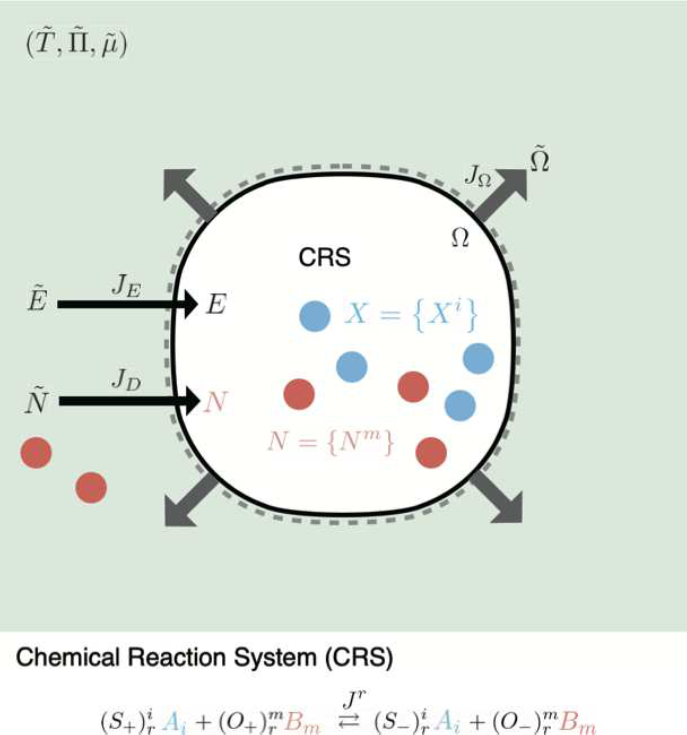
\includegraphics[width=7cm]{crs.png}
  \caption{考えている系の概略図(出典は論文)}
  \label{fig:crs}
\end{figure}

膜に囲まれた系が浴の中に置かれているとし,その膜を透過できる物質(open chemicalsと呼ぶ)$m=1,2,\cdots,\mathcal{N}_N$と透過できない物質(confined chemicalsと呼ぶ)$i=1,2,\cdots,\mathcal{N}_X$が存在すると考える.
この系は浴とエネルギーやopen chemicalsをやりとりでき,体積も変動しうるとする.
また,系の内部は常によく撹拌されていると仮定し,それによって系の状態は,系のエネルギー$E$,体積$\Omega$,open chemicalsの粒子数$N=\{ N^m \}$,confined chemicalsの粒子数$X = \{ X^i \}$の組$(E,\Omega,N,X)$により一意に指定できると考える.

一方で,浴には温度$\tilde{T}$,圧力$\tilde{\Pi}$,open chemicals $N=\{ N^m \}$に対する化学ポテンシャル$\tilde{\mu} = \{ \tilde{\mu}_m \}$が与えられているとする.
また,浴のエネルギー,体積,open chemicalsの粒子数をそれぞれ$\tilde{E}$,$\tilde{\Omega}$,$\tilde{N} = \{ \tilde{N}^m \}$と書く.
ただし,浴にはconfined chemicalsは存在しないとする.

また,物質間に化学反応$r=1,2,\cdots,\mathcal{N}_R$が起こると考える.
この化学反応全体のstoichiometric matrixのうち,open chemicalsの行だけを取り出した小行列を$O=(O^m_r)$,confined chemicalsの行だけを取り出した小行列を$S=(S^i_r)$とする.
そして$S$をautocatalytic coreと考え,その正則性を仮定する.(つまり$\mathcal{N}_X=\mathcal{N}_R=\mathrm{rank}(S)$が成り立つとする\footnote{この仮定は余分な反応が1個でも増えると崩れるが,その場合であってもしっかりと議論すればこの論文と同様の結果が得られるという予想のもと研究が進められているらしい.}.)

以上の状況から,系の状態変化を微分方程式で書くと,
\begin{align}
  \dv{E}{t} &= J_{E}(t) \\
  \dv{\Omega}{t} &= J_{\Omega}(t) \\
  \dv{N^m}{t} &= O^m_r J^r(t) + J^m_{D}(t) \\
  \dv{X^i}{t} &= S^i_r J^r(t)
\end{align}
となる\footnote{アインシュタインの規約を用いている.}.
ここで,$J_{E}(t)$,$J_{\Omega}(t)$,$J_{D}(t)=\{ J^m_{D}(t) \}$はそれぞれ単位時間あたりの浴から系へのエネルギー,体積,open chemicalsの流入量を指し,$J(t) = \{ J^r(t) \}$は単位時間あたりの反応ベクトルを指す.

ここで,反応は十分遅く
\begin{equation}
  J_{E}(t), J_{\Omega}(t), J_{D}(t) \gg J(t)
\end{equation}
という関係が成り立つと仮定する\footnote{発表時,「生物の系において化学反応よりも体積の変化がはるかに速いとは考えにくいので,この仮定には疑問が残る」という議論があった.}.
このとき系の振る舞いは,時間スケールの異なる次の二つの過程に分離することができる.
\begin{enumerate}
  \item 化学反応を待たずに$(E,\Omega,N)$が熱力学的な平衡状態に到達する素早い過程(fast dynamics)
  \item Fast dynamicsで指定される限られた状態空間に拘束されながら,化学反応により系の状態が変化する遅い過程(slow dynamics)
\end{enumerate}

これ以降では,fast dynamicsによってたどり着く状態を準平衡状態(quasi-equilibrium state)と呼び,そのときの系のパラメータには``QEQ''という添字をつける.

\subsection{Fast dynamicsの解析}
まず,fast dynamicsによって系の状態がどのように制限されるかを考える.
Fast dynamicsでは化学反応を考えないので,単純な熱力学を適用できる.
具体的には,浴と系のやりとりから
\begin{align}
  d\tilde{E} &= - dE \\
  d\tilde{\Omega} &= - d\Omega \\
  d\tilde{N}^m &= - dN^m  
\end{align}
がいえる.
次に,系のエントロピーを$\Sigma$,浴のエントロピーを$\tilde{\Sigma}$とすると,全系のエントロピー$\Sigma^{\mathrm{tot}}$ついて
\begin{equation}
  d\Sigma^{\mathrm{tot}} =  d\Sigma + d\tilde{\Sigma} \ge 0
\end{equation}
がいえる(熱力学第2法則).
また,系とやりとりするエネルギー,体積,open chemicalsの粒子数はいずれも浴にとっては小さいので,浴は常に平衡状態にあると考え,熱力学第1法則から
\begin{equation}
  d\tilde{E} = \tilde{T}d\tilde{\Sigma} - \tilde{\Pi}d\tilde{\Omega} + \tilde{\mu}_m d\tilde{N}^m
\end{equation}
が成り立つとして良い.
また,グランドポテンシャル
\begin{equation}
  \Phi = E - \tilde{T} \Sigma - \tilde{\mu}_m N^m
\end{equation}
を用いると,
\begin{align}
  d\Phi &= dE - \tilde{T} d\Sigma - \Sigma d\tilde{T} - \tilde{\mu}_m dN^m - N^m d\tilde{\mu}_m \notag\\
  &= -d\tilde{E} - \tilde{T} d\Sigma - \Sigma d\tilde{T} + \tilde{\mu}_m d\tilde{N}^m - N^m d\tilde{\mu}_m \notag\\
  &\le -d\tilde{E} + \tilde{T} d\tilde{\Sigma} - \Sigma d\tilde{T} + \tilde{\mu}_m d\tilde{N}^m - N^m d\tilde{\mu}_m \notag\\
  &= - \Sigma d\tilde{T} + \tilde{\Pi}d\tilde{\Omega} - N^m d\tilde{\mu}_m \notag\\
  &=   - \Sigma d\tilde{T} - \tilde{\Pi}d\Omega - N^m d\tilde{\mu}_m \label{grand}
\end{align}
よって,$\tilde{T}$,$\tilde{\mu}_m$一定のもとで
\begin{equation}
  d\left(\Phi + \Pi \Omega \right) \le 0
\end{equation}
がいえる.
ゆえに$\Phi + \Pi \Omega$は準平衡状態では最小となる.
ここで,グランドポテンシャルの正確な定義は
\begin{equation}
  \Phi [\tilde{T}, \tilde{\mu}; \Omega, X] = \min_{E, N} \left\{ E - \tilde{T} \Sigma[E, \Omega, N, X] - \tilde{\mu}_m N^m \right\}
\end{equation}
なので,$\Phi + \Pi \Omega$を最小化するときに動かす変数は$\Omega$である\footnote{浴のパラメータはもちろん一定だが,fast dynamicsでは化学反応がないので$X$も一定である.}.
したがって,fast dynamicsの結果,最終的な体積は
\begin{equation}
  \Omega_{\mathrm{QEQ}}(X) = \mathrm{arg}\min_{\Omega} \left\{ \Phi [\tilde{T}, \tilde{\mu}; \Omega, X]  + \tilde{\Pi} \Omega \right\}
\end{equation}
となる\footnote{発表はここで中断したが,きりが悪いので資料ではもう少し話を続ける.もちろん2回目の発表はこの続きから行う.}.
この式は2回目の発表で重要な役割を果たす.

また,準平衡状態では式\eqref{grand}より
\begin{align}
  \Sigma_{\mathrm{QEQ}}(X) &= - \pdv{\Phi [\tilde{T}, \tilde{\mu}; \Omega_{\mathrm{QEQ}}, X]}{\tilde{T}} \\
  N^m_{\mathrm{QEQ}}(X) &= - \pdv{\Phi [\tilde{T}, \tilde{\mu}; \Omega_{\mathrm{QEQ}}, X]}{\tilde{\mu}_m}
\end{align}
が成り立つ.
これらをグランドポテンシャルの定義式に代入して
\begin{equation}
  E_{\mathrm{QEQ}}(X) = \Phi [\tilde{T}, \tilde{\mu}; \Omega_{\mathrm{QEQ}}, X] - \tilde{T} \pdv{\Phi [\tilde{T}, \tilde{\mu}; \Omega_{\mathrm{QEQ}}, X]}{\tilde{T}} - \tilde{\mu}_m \pdv{\Phi [\tilde{T}, \tilde{\mu}; \Omega_{\mathrm{QEQ}}, X]}{\tilde{\mu}_m}
\end{equation}
がいえる.
こうして,fast dynamicsで収束する準平衡状態$(E_{\mathrm{QEQ}}(X), \Omega_{\mathrm{QEQ}}(X), N_{\mathrm{QEQ}}(X))$が求まった.

\subsection{Slow dynamicsの解析}
Slow dynamicsでは化学反応も考える.
しかしfast dynamicsのため系の状態は準平衡状態に拘束されるので,微分方程式は次のようになる.
\begin{align}
  \dv{X^i}{t} &= S^i_r J^r(t) \\
  \dv{\tilde{E}}{t} &= - \dv{E_{\mathrm{QEQ}}(X)}{t} \\
  \dv{\tilde{\Omega}}{t} &= - \dv{\Omega_{\mathrm{QEQ}}(X)}{t} \\
  \dv{\tilde{N}^m}{t} &= O^m_r J^r(t) - \dv{N^m_{\mathrm{QEQ}}(X)}{t}
\end{align}
ここで,$S$は正則と仮定したので
\begin{equation}
  J^r(t) dt = (S^{-1})^r_i dX^i 
\end{equation}
がいえ,
\begin{equation}
  d\tilde{N}^m = O^m_r J^r(t) dt - dN^m_{\mathrm{QEQ}}(X) = O^m_r (S^{-1})^r_i dX^i - dN^m_{\mathrm{QEQ}}(X)
\end{equation}
と書ける.
したがって,全系のエントロピーについて
\begin{align}
  d\Sigma^{\mathrm{tot}} &= d\Sigma_{\mathrm{QEQ}} + d\tilde{\Sigma} \notag\\
  &= d\Sigma_{\mathrm{QEQ}} + \frac{1}{\tilde{T}} d\tilde{E} + \frac{\tilde{\Pi}}{\tilde{T}} d\tilde{\Omega} - \frac{\tilde{\mu}_m}{\tilde{T}} d\tilde{N}^m \notag\\
  &= d\Sigma_{\mathrm{QEQ}} - \frac{1}{\tilde{T}} dE_{\mathrm{QEQ}} - \frac{\tilde{\Pi}}{\tilde{T}} d\Omega_{\mathrm{QEQ}} + \frac{\tilde{\mu}_m}{\tilde{T}} dN^m_{\mathrm{QEQ}} - \frac{\tilde{\mu}_m}{\tilde{T}} O^m_r (S^{-1})^r_i dX^i \notag\\
  &= d\Sigma_{\mathrm{QEQ}} - \frac{1}{\tilde{T}} dE_{\mathrm{QEQ}} - \frac{\tilde{\Pi}}{\tilde{T}} d\Omega_{\mathrm{QEQ}} + \frac{\tilde{\mu}_m}{\tilde{T}} dN^m_{\mathrm{QEQ}} + \frac{y_i^{\mathrm{EQ}}}{\tilde{T}} dX^i 
\end{align}
が成り立つ.
ここで
\begin{equation}
  y_i^{\mathrm{EQ}} = - \tilde{\mu}_m O^m_r (S^{-1})^r_i
\end{equation}
と定義した.
したがって,全系のエントロピーはグランドポテンシャルを用いて
\begin{align}
  \Sigma^{\mathrm{tot}} &= \Sigma_{\mathrm{QEQ}} - \frac{1}{\tilde{T}} E_{\mathrm{QEQ}} - \frac{\tilde{\Pi}}{\tilde{T}} \Omega_{\mathrm{QEQ}} + \frac{\tilde{\mu}_m}{\tilde{T}} N^m_{\mathrm{QEQ}} + \frac{y_i^{\mathrm{EQ}}}{\tilde{T}} X^i + const. \notag\\
  &= - \frac{1}{\tilde{T}} \left\{ \Phi[\tilde{T}, \tilde{\mu}; \Omega, X] + \tilde{\Pi}\Omega_{\mathrm{QEQ}} - y_i^{\mathrm{EQ}} X^i \right\} + const.
\end{align}
と書ける.
2回目の発表では,この表式をもとに全系のエントロピーを最大化するような$X$を考える.

\end{document}